\documentclass[12pt,norsk,a4paper]{article}
\usepackage{graphicx}
\usepackage{verbatim}
\usepackage{hyperref}
\usepackage{float}
\usepackage{amsmath}
\usepackage{amsfonts}
\usepackage{ulem}
\usepackage{multirow}
\newcommand*\xor{\mathbin{\oplus}}
\usepackage[utf8]{inputenc}
\usepackage[norsk]{babel}

\begin {document}
\title{Matte 3 - Øving 13}
\author {Arve Nygård}

\maketitle

\clearpage

\section{Oppgave 1}
\subsection{Deloppgave 1}
\begin{center}
$w= -8 + 8 \sqrt{3}i$\\[0.5cm]
$r = \sqrt{(-8)^2 + (8 \sqrt{3})^2} = \sqrt{4* 64} = 16    $\\[0.5cm]
$\phi = \arctan(\frac{8 \sqrt{3} }{-8}) = \arctan(- \sqrt{3}) = \frac{-\pi}{3}$\\[0.5cm]
Vi er i 2. kvadrant, så vi har at $\theta = \frac{-\pi}{3} + \pi = \mathbf{\frac{2\pi}{3} }$\\[0.5cm]
$\uuline{w = 16(\cos(\frac{2\pi}{3}) - i \sin(\frac{2\pi}{3}))}$
\end{center}
\subsection{Deloppgave 2} % (fold)
\label{sub:deloppgave_2}
Vi skal finne fjerderøttene. Det er 4 av disse, og de ligger 90 grader på hverandre.

1. rot:
\begin{center}
$w^{1/4} = 16^{1/4}\Bigg[\cos(\frac{1}{4} \frac{2\pi}{3}) + i \sin(\frac{1}{4} \frac{2\pi}{3})\Bigg] = 2\Bigg[\cos(\frac{\pi}{6}) + i \sin(\frac{\pi}{6})\Bigg]$ \\
$= \uuline{\mathbf{\sqrt{3}+i }}$
\end{center}

2. rot:\\
Radien er alltid den samme, vi legger på $\frac{\pi}{2}$.
\begin{center}

$2\Bigg[ \cos(\frac{\pi}{6} + \frac{\pi}{2}) + i \sin(\frac{\pi}{6} + \frac{\pi}{2}) \Bigg] = 2\cos(\frac{2\pi}{3}) + 2 \sin(\frac{2\pi}{3})$\\
$ = \mathbf{\uuline{-1 + \sqrt{3} i }}$
\end{center}
3.- og 4. rot finner vi ved inspeksjon: Enten av tegning eller tallene. Vi skal ha én rot i hver kvadrant.
\begin{center}
3. rot:
$\mathbf{\uuline{- \sqrt{3} - i }}$ \hspace{2cm}
4. rot:
$\mathbf{\uuline{1 -\sqrt{3} i }}$
\end{center}

% subsection deloppgave_2 (end)

\clearpage
\section{Oppgave 2} % (fold)
\label{sec:oppgave_2}
\subsection{a)}

\begin{center}
$y'' + 4y' + 5y = 0 \hspace{1cm} , \hspace{1cm} y(0) = 1 , y'(0) = 2$\\[1cm]
$\lambda^2 + 4\lambda + 5 = 0$ \\
$\Longrightarrow \lambda_1 = -2 -i , \hspace{1cm} \lambda_2 = -2 + i$\\
\end{center}
Vi får imaginære tall, og dermed blir y(x) på formen $C_1 e^{-2x} \cos(x) + C_2 e^{-2x} \sin(x)$.\\
Vi setter x=0 og løser for $C_1$:
\begin{center}
$y(0) = 1 = C_1 e^0 \cos0 + C_2 e^0 \sin0$\\
$1 = C_1 \cdot 1 \cdot 1 + C_2 \cdot 1 \cdot 0$\\
$\mathbf{C_1 = 1}$
\end{center}
Vi har nå at \hspace{2cm} $y(x) = e^{-2x}\cos x + C_2 e^{-2x} \sin x$.\\
Deriver uttrykket, bruk initialverdi og løs for $C_2$:
\begin{center}
$y'(x) = C_2\Bigg[e^{-2x}\sin x \Bigg]' + \Bigg[ e^{-2x} \cos x \Bigg]'$ \\
$= C_2\Bigg[-2e^{-2x}\sin x  + e^{-2x} \cos x\Bigg] + \Bigg[ -2e^{-2x} \cos x - e^{-2x}\sin x \Bigg]$ \\
$= C_2e^{-2x} \Bigg[ -2 \sin x + \cos x \Bigg] + e^{-2x} \Bigg[ -2 \cos x - \sin x\Bigg]$
\end{center}
Vi setter så inn x=0:
\begin{center}
$y'(0) = 2 = C_2 e^0 \Bigg[ -2 \sin 0 + \cos 0\Bigg] + e^0 \Bigg[ -2 \cos 0 - \sin 0 \Bigg] $\\
$ 2 = C_2 \bigg[ 1 \bigg] + \bigg[ -2 \bigg]$\\
$2 = C_2 -2 $\\
$\mathbf{C_2 = 4}$
\end{center}

Vi har nå hele løsningen på initialverdiproblemet: 
\begin{center}
$y(x) = e^{-2x} \cos x + 4 e^{-2x} \sin x = \mathbf{\uuline{e^{2x} \big(\cos x + 4 \sin x \big)}}$
\end{center}
\clearpage

\subsection{b)} % (fold)
\label{sub:2_b_}
Fra oppgave 2a har vi at $y_h = e^{2x} \big(\cos x + 4 \sin x \big)$.\\
Vi leter etter en partikulær løsning på formen $y_p = A \cos x + B \sin x + Cx + D$.\\
\begin{center}
$y_p = A \cos x + B \sin x + Cx + D$\\
$y'_p = -A \sin x + B \cos x + C$\\
$y''_p = -A \cos x - B \sin x$\\[1cm]
\end{center}
Vi setter opp stykket, og setter inn vår partikulærløsning, og løser deretter for A, B, C og D:
\begin{center}
$y'' + 4y' + 5y = 4 \cos x + 5 x$\\
$\big(4A + 4B\big) \cos x + \big( 4B -4 A\big) \sin x + Cx + d = 4 \cos x + 5 x$\\
\end{center}
Vi løser for A og B:
\begin{center}
$4A + 4B = 4$\\
$4B - 4A = 0$\\
$\Rightarrow A = \frac{1}{2} , B = \frac{1}{2}$
\end{center}
Vi løser så for C og D:
\begin{center}
$4C + 5Cx + 5D = 5x \Rightarrow C = 1$\\
$4 + 5D = 0 \Rightarrow D = \frac{-4}{5}$
\end{center}

Vi har nå en fullstendig partikulærløsning:
\begin{center}
$y_p = \frac{1}{2} \cos x + \frac{1}{2} \sin x = x - \frac{4}{5}$
\end{center}
Den generelle løsningen blir da:
\begin{center}
$y_g = y_h = y_g$\\[0.3cm]
$\mathbf{\uuline{y_g = e^{-2x} \bigg(\cos x + 4 \sin x \bigg) + \frac{1}{2}\bigg( \cos x + \sin x \bigg) + x - \frac{4}{5}}}$
\end{center}
% subsection 2_b_ (end)
\subsection{c)} % (fold)
\label{sub:c_}
Denne klarte jeg ikke :(
% subsection c_ (end)
% section oppgave_2 (end)
\clearpage
\section{Oppgave 3} % (fold)
\label{sec:oppgave_3}
\subsection{a)} % (fold)
\label{sub:a_}
\uuline{Alternativ C}
\subsection{b)}
\uuline{Alternativ A}
\clearpage
\section{Oppgave 4} % (fold)
\label{sec:oppgave_4}
\subsection{a)} % (fold)
\label{sub:a_}

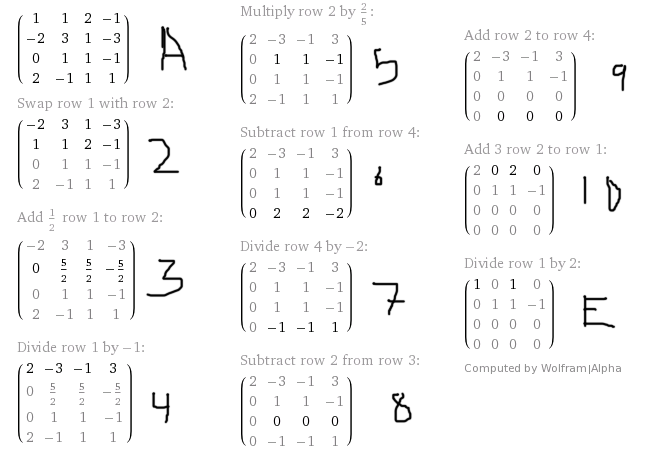
\includegraphics[scale=0.4]{row-reduce.png}\\
Basis for $Col A$: {$\vec{v_1}, \vec{v_2}$}\\
\begin{equation*}
\begin{Bmatrix}
\begin{bmatrix}
1\\
-2\\
0\\
2
\end{bmatrix} & , &
\begin{bmatrix}
1\\
3\\
1\\
-1
\end{bmatrix}
\end{Bmatrix}
\end{equation*}
Basis for $Row A$:
\begin{equation*}
\begin{Bmatrix}
\begin{bmatrix}
1 & 0 & 1 & 0
\end{bmatrix}\\
,\\
\begin{bmatrix}
1 & 0 & 1 & -1
\end{bmatrix}
\end{Bmatrix}
\end{equation*}
\clearpage
\subsubsection{b)} % (fold)
\label{ssub:b_}
$Nul A$:

\begin{equation*}
\begin{bmatrix}
1&0&1&0&|&0\\
0&1&1&-1&|&0\\
0&0&0&0&|&0\\
0&0&0&0&|&0
\end{bmatrix}
\end{equation*}
\[x_1 = -x_3\]
\[x_2 = -x_3 + x_4\]
\[x_3, x_4 \textrm{ fri.} \]

\begin{equation*}
\begin{bmatrix}
x_1\\ x_2\\ x_3\\ x_4\\
\end{bmatrix} 
= 
x3 
\begin{bmatrix}
-1\\ -1\\ 1\\ 0\\ 
\end{bmatrix} 
+ x_4
\begin{bmatrix}
0\\ 1\\ 0\\ 1\\ 
\end{bmatrix} 
\Rightarrow 
\textrm{Nul A} = 
\left\{{
\begin{bmatrix}
-x\\ y-x\\ x\\ y\\ 
\end{bmatrix} | x, y \in \mathbb{R}}\right\}
\end{equation*}
For at $A\vec{x} = \vec{b}$ skal ha en løsning, må $\vec{b} $ være i $Col A$.\\
Siden $b_1$ og $b_2$ er gitt, kan vi finne hvilken kombinasjon av kollonnevektorer i $A$ som $\vec{b} $ består av. Vi fokuserer på rad 1 og 2; siden disse er gitt for $\vec{b}$.\\
\\
Vi må finne $a$ og $b$ slik at $a + b = 1$, og $-2a + 3b = 0$

\begin{equation*}
\begin{bmatrix}
1&1&|&1\\
-2 & 3&|& 0
\end{bmatrix}
\sim
\begin{bmatrix}
1&0&|& \frac{3}{5}\\ 
0&1&|& \frac{2}{5}\\ 
\end{bmatrix}
\end{equation*}
Dermed har vi at $a = \frac{3}{5} $ og $b = \frac{2}{5}$. Dette betyr at $\vec{b}$ består av $\frac{3}{5} \vec{v_1} + \frac{2}{5}\vec{v_2}$, der $\vec{v_1}$ og $\vec{v_2}$ er vektorene i $Col A$.
Da gjenstår bare litt enkel regning for å finne $\alpha $ og $ \beta$:
\begin{equation*}
\alpha = \frac{3}{5} \cdot 0 + \frac{2}{5} \cdot 1 = \mathbf{\uuline{\frac{2}{5}}}
\end{equation*}
\begin{equation*}
\beta = \frac{3}{5} \cdot 2 + \frac{2}{5} \cdot -1 = \mathbf{\uuline{\frac{4}{5}}}
\end{equation*}
\clearpage


\subsection{c)} % (fold)
\label{sub:c_}
\[\vec{v_1} = \vec{u_1}\]
\[\tilde{v_2} = \vec{u_2} - \left(\frac{\vec{u_2} \cdot \vec{v_1}}{\vec{v_1}\cdot\vec{v_1}}\right)\vec{v_1} = 
\begin{bmatrix}
0\\1\\1\\-1
\end{bmatrix}
- \frac{1}{2}
\begin{bmatrix}
1\\0\\1\\0 
\end{bmatrix}
= \frac{1}{2} 
\begin{bmatrix}
-1\\2\\1\\-2
\end{bmatrix}, \hspace{0.5cm} \vec{v_2} = (-1,2,1,-2)
 \]

\section{Oppgave 5} % (fold)
\label{sec:oppgave_5}
Vi ser på den karakteristiske likningen $det(A - I) = 0$:
\[
\begin{vmatrix}
3-\lambda & 4 & -2\\
-2 & -3-\lambda & 2\\
0&0& 1-\lambda
\end{vmatrix}
= (1-\lambda)
\begin{vmatrix}
3-\lambda & 4\\
-2 & -3-\lambda
\end{vmatrix}
= (1-\lambda)(\lambda^2 -1) = -(\lambda-1)^2(\lambda +1) = 0
\]

Dermed er egenverdiene til $A$ $1$ og $-1$
% section oppgave_5 (end)

\end{document}